\documentclass{article}
\usepackage{tikz}
\usetikzlibrary{positioning}

\begin{document}
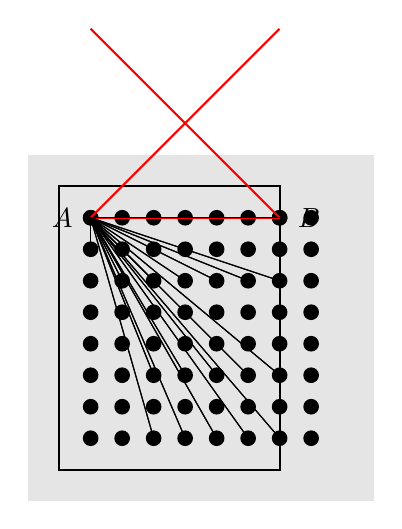
\begin{tikzpicture}[scale=0.4]
    \fill[gray!20] (-3,-3) rectangle (8,8);
    
    % Left diagram
    \draw[thick] (-2,-2) -- (-2,7) -- (5,7) -- (5,-2) -- cycle;
    \foreach \x in {-1,0,...,6} {
        \foreach \y in {-1,0,...,6} {
            \node[circle,fill,inner sep=2pt] at (\x,\y) {};
        }
    }
    \node[circle,fill,inner sep=2pt,label=left:$A$] at (-1,6) {};
    \node[circle,fill,inner sep=2pt,label=right:$B$] at (5,6) {};
    \draw[red, thick] (-1,6) -- (5,6);
    \foreach \x/\y in {-1/5, 0/4, 1/4, 2/4, 3/4, 4/4, 5/4, -1/6, 0/6, 1/6, 2/6, 3/6, 4/6, 5/6, 1/1, 2/1, 3/1, 4/1, 5/1, 1/-1, 2/-1, 3/-1, 4/-1, 5/-1} {
        \draw (-1,6) -- (\x,\y);
    }

    % Right diagram
    \draw[thick, red, thick,domain=-1:5,samples=200] plot (\x,{\x+7});
    \draw[thick, red, thick,domain=-1:5,samples=200] plot (\x,{-(\x-5)+6});
    \foreach \x/\y in {-1/5, 0/4, 1/4, 2/4, 3/4, 4/4, 5/4, -1/6, 0/6, 1/6, 2/6, 3/6, 4/6, 5/6, 1/1, 2/1, 3/1, 4/1, 5/1, 1/-1, 2/-1, 3/-1, 4/-1, 5/-1} {
        \draw (-1,6) -- (\x,\y);
    }
\end{tikzpicture}